\documentclass[11pt]{article}

\author{wilricknl}
\title{3D Math Primer - Solutions chapter 11}

\usepackage{amsmath}
\usepackage{amssymb}
\usepackage{float}
\usepackage{enumerate}
\usepackage{graphicx}
\usepackage{url}

\begin{document}

\maketitle

\section{Solutions chapter 11}

\subsection{Exercise 1}

$$\frac{1\text{lb}}{\text{in}^2} \times \frac{4.448\text{N}}{1\text{lb}} \times \left(\frac{\text{in}}{0.0254\text{m}}\right)^2=\frac{4.448\text{N}}{(0.0254\text{m})^2} = \frac{6894.4\text{N}}{\text{m}^2}$$

\subsection{Exercise 2}

\begin{figure}[H]
\centering
    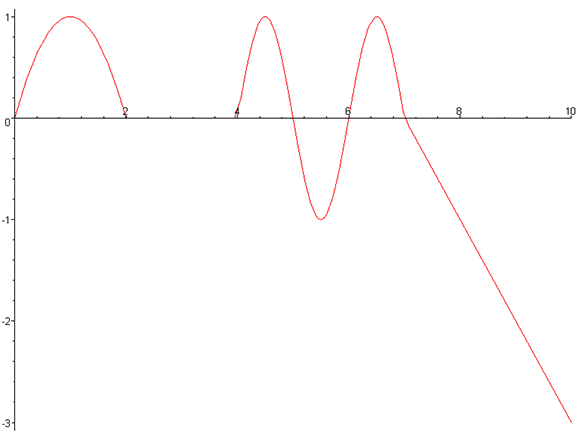
\includegraphics[width=0.6\textwidth]{exercise02}
\caption{Graph of velocity}
\label{fig:velocity-graph}
\end{figure}

\subsection{Exercise 3}

\begin{enumerate}[a.]
	\item $\frac{x(1)-x(0)}{1-1} = 1$
	\item $\frac{x(2)-x(1)}{2-1} = -1$
	\item $\frac{x(2)-x(0)}{2-0} = 0$
	\item $\frac{x(6.5)-x(5.5)}{6.5-5.5} = 2$
	\item $\frac{x(9)-x(0)}{9-0} = \frac{2}{9}$
\end{enumerate}

\subsection{Exercise 4}

\begin{equation*}
	v(t) =
	\begin{cases}
		2-2t & 0 < t < 2 \\
		0 & 2 < t < 4 \\
		\pi \cos(\pi t) & 4 < t < 7 \\
		-1 & 7 < t
	\end{cases}
\end{equation*}

\subsection{Exercise 5}

\begin{enumerate}[a.]
	\item $2-2 \cdot{} 0.1 = 1.8$
	\item $2-2 = 0$
	\item $2-3.8 = -1.8$
	\item $\pi \cdot \cos(4.1\pi) = 2.98 \dots $
	\item $\pi \cdot \cos(5\pi) = \pi$
	\item $\pi \cdot \cos(6.5\pi) = 0$
	\item $-1$
	\item $-1$
\end{enumerate}

\subsection{Exercise 6}

\begin{equation*}
	a(t) =
	\begin{cases}
		-2 & 0 < t < 2 \\
		0 & 2 < t < 4 \\
		-\pi^2 \sin(\pi t) & 4 < t < 7 \\
		0 & 7 < t
	\end{cases}
\end{equation*}

\subsection{Exercise 7}

\begin{enumerate}[a.]
	\item $-2$
	\item $-2$
	\item $-2$
	\item $-3.0498 \dots$
	\item $0$
	\item $-9.8690 \dots$
	\item $0$
	\item $0$
\end{enumerate}

\subsection{Exercise 8}

Zero if stationary, the other one I don't understand.

\subsection{Exercise 9}

\begin{enumerate}[a.]
	\item % a
		\begin{itemize}
			\item $\textbf{v}_0 = \textbf{p}_0 = (\dot{x}_0, \dot{y}_0)$
			\item $\dot{x}_0 = 150 \cos (40^{\circ}) = 114.90$
			\item $\dot{y}_0 = 150 \sin (40^{\circ}) = 96.41$
			\item $(114.90, 96.41) \text{ft/s}$
		\end{itemize}
	\item % b
		$t = \frac{-96.41}{-32\text{ft/2}^2} = 3.01\text{s}$
	\item % c
		\begin{itemize}
			\item $x = (3.01)(114.9) = 345.845$
			\item $y = (3.01)(96.41) + \frac{1}{2}(-32)(3.01^2) = 145.23$
			\item $(345.845 + 0, 145.23 + 10) = (345.845, 155.23)$
		\end{itemize}
	\item % d
		Twice the apex, so $6.02\text{s}$.
	\item % e
		$(345.845)(2) = 691.698 \text{ft}$
\end{enumerate}

\subsection{Exercise 10}

% bruh, so much latex
\begin{align*}
0 &= \textbf{a} \cdot{} \frac{\textbf{a}}{2} \cdot{} t^2 + (\textbf{v}_0 \cdot{} \textbf{a})t - (\bigtriangleup \textbf{p} \cdot{} \textbf{a}) \\
t &= \frac{-(\textbf{v}_0 \cdot{} \textbf{a}) \pm \sqrt{((\textbf{v}_0 \cdot{} \textbf{a})^2+2(\textbf{a} \cdot \textbf{a})(\bigtriangleup \textbf{p} \cdot{} \textbf{a})}}{\textbf{a} \cdot{} \textbf{a}}
\end{align*}

\subsection{Exercise 11}

\begin{align*}
e^{ix} &= 1 + \frac{ix}{1!} + \frac{(ix)^2}{2!} + \frac{(ix)^3}{3!} + \frac{(ix)^4}{4!} + \frac{(ix)^5}{5!} + \dots \\
&= 1 + i\frac{x}{1!} - \frac{(x)^2}{2!} - i\frac{(x)^3}{3!} + \frac{(x)^4}{4!} + i\frac{(x)^5}{5!} + \dots \\
&= (1 - \frac{(x)^2}{2!} + \frac{(x)^4}{4!} + \dots{}) + i(x - \frac{(x)^3}{3!} + \frac{(x)^5}{5!} + \dots) \\
&= \cos x + i \sin x
\end{align*}

Euler's formula: $e^{i \pi}+ 1 = 0$.

\subsection{Exercise 12}

\begin{itemize}
	\item $\text{radius} = 6371\text{km} + 340\text{km} = 6711\text{km}$
	\item $\text{circumference} = (2\pi)(\text{radius}) = (2\pi)(6711\text{km}) = 42166.45\text{km}$
	\item $\text{speed} = 27740\text{km/h} = 7705.5\text{m/s}$
	\item $\text{orbital period} = \frac{42166.45\text{km}}{27740\text{km/h}} = 1.52\text{h} = (1.52)(60) \approx 91\text{min}$
	\item $a = \frac{s^2}{r} = \frac{7705.5 \text{m}/\text{s}^2}{6711000\text{m}} = 8.847\text{m}/\text{s}^2$
\end{itemize}

\end{document}
